\documentclass[11pt]{article}
\usepackage{latexsym}
\usepackage{amsmath}
\usepackage{amssymb}
\usepackage{amsthm}
\usepackage{epsfig}
\usepackage[tight]{subfigure}

\usepackage{amsmath}

\DeclareMathOperator*{\minimize}{min}
\DeclareMathOperator*{\maximize}{max}

\usepackage{algorithm}
 %on linux you may need to run sudo apt-get install texlive-full to install algorithm.sys
\usepackage{algorithmic}

\usepackage{verbatim}

%%%%%%%%%%%%%%%%%%%%%%%%%%%%%%%%%%%%%%%%%%
% Custom commands                        %
%%%%%%%%%%%%%%%%%%%%%%%%%%%%%%%%%%%%%%%%%%

\newcommand{\vc}[1]{\boldsymbol{#1}}
\newcommand{\adj}[1]{\frac{d J}{d #1}}
\newcommand{\chain}[2]{\adj{#2} = \adj{#1}\frac{d #1}{d #2}}

% mathcal
\newcommand{\Ac}{\mathcal{A}}
\newcommand{\Bc}{\mathcal{B}}
\newcommand{\Cc}{\mathcal{C}}
\newcommand{\Dc}{\mathcal{D}}
\newcommand{\Ec}{\mathcal{E}}
\newcommand{\Fc}{\mathcal{F}}
\newcommand{\Gc}{\mathcal{G}}
\newcommand{\Hc}{\mathcal{H}}
\newcommand{\Ic}{\mathcal{I}}
\newcommand{\Jc}{\mathcal{J}}
\newcommand{\Kc}{\mathcal{K}}
\newcommand{\Lc}{\mathcal{L}}
\newcommand{\Mc}{\mathcal{M}}
\newcommand{\Nc}{\mathcal{N}}
\newcommand{\Oc}{\mathcal{O}}
\newcommand{\Pc}{\mathcal{P}}
\newcommand{\Qc}{\mathcal{Q}}
\newcommand{\Rc}{\mathcal{R}}
\newcommand{\Sc}{\mathcal{S}}
\newcommand{\Tc}{\mathcal{T}}
\newcommand{\Uc}{\mathcal{U}}
\newcommand{\Vc}{\mathcal{V}}
\newcommand{\Wc}{\mathcal{W}}
\newcommand{\Xc}{\mathcal{X}}
\newcommand{\Yc}{\mathcal{Y}}
\newcommand{\Zc}{\mathcal{Z}}

% mathbb
\newcommand{\Ab}{\mathbb{A}}
\newcommand{\Bb}{\mathbb{B}}
\newcommand{\Cb}{\mathbb{C}}
\newcommand{\Db}{\mathbb{D}}
\newcommand{\Eb}{\mathbb{E}}
\newcommand{\Fb}{\mathbb{F}}
\newcommand{\Gb}{\mathbb{G}}
\newcommand{\Hb}{\mathbb{H}}
\newcommand{\Ib}{\mathbb{I}}
\newcommand{\Jb}{\mathbb{J}}
\newcommand{\Kb}{\mathbb{K}}
\newcommand{\Lb}{\mathbb{L}}
\newcommand{\Mb}{\mathbb{M}}
\newcommand{\Nb}{\mathbb{N}}
\newcommand{\Ob}{\mathbb{O}}
\newcommand{\Pb}{\mathbb{P}}
\newcommand{\Qb}{\mathbb{Q}}
\newcommand{\Rb}{\mathbb{R}}
\newcommand{\Sb}{\mathbb{S}}
\newcommand{\Tb}{\mathbb{T}}
\newcommand{\Ub}{\mathbb{U}}
\newcommand{\Vb}{\mathbb{V}}
\newcommand{\Wb}{\mathbb{W}}
\newcommand{\Xb}{\mathbb{X}}
\newcommand{\Yb}{\mathbb{Y}}
\newcommand{\Zb}{\mathbb{Z}}

% mathbf lowercase
\newcommand{\av}{\mathbf{a}}
\newcommand{\bv}{\mathbf{b}}
\newcommand{\cv}{\mathbf{c}}
\newcommand{\dv}{\mathbf{d}}
\newcommand{\ev}{\mathbf{e}}
\newcommand{\fv}{\mathbf{f}}
\newcommand{\gv}{\mathbf{g}}
\newcommand{\hv}{\mathbf{h}}
\newcommand{\iv}{\mathbf{i}}
\newcommand{\jv}{\mathbf{j}}
\newcommand{\kv}{\mathbf{k}}
\newcommand{\lv}{\mathbf{l}}
\newcommand{\mv}{\mathbf{m}}
\newcommand{\nv}{\mathbf{n}}
\newcommand{\ov}{\mathbf{o}}
\newcommand{\pv}{\mathbf{p}}
\newcommand{\qv}{\mathbf{q}}
\newcommand{\rv}{\mathbf{r}}
\newcommand{\sv}{\mathbf{s}}
\newcommand{\tv}{\mathbf{t}}
\newcommand{\uv}{\mathbf{u}}
\newcommand{\vv}{\mathbf{v}}
\newcommand{\wv}{\mathbf{w}}
\newcommand{\xv}{\mathbf{x}}
\newcommand{\yv}{\mathbf{y}}
\newcommand{\zv}{\mathbf{z}}

% mathbf uppercase
\newcommand{\Av}{\mathbf{A}}
\newcommand{\Bv}{\mathbf{B}}
\newcommand{\Cv}{\mathbf{C}}
\newcommand{\Dv}{\mathbf{D}}
\newcommand{\Ev}{\mathbf{E}}
\newcommand{\Fv}{\mathbf{F}}
\newcommand{\Gv}{\mathbf{G}}
\newcommand{\Hv}{\mathbf{H}}
\newcommand{\Iv}{\mathbf{I}}
\newcommand{\Jv}{\mathbf{J}}
\newcommand{\Kv}{\mathbf{K}}
\newcommand{\Lv}{\mathbf{L}}
\newcommand{\Mv}{\mathbf{M}}
\newcommand{\Nv}{\mathbf{N}}
\newcommand{\Ov}{\mathbf{O}}
\newcommand{\Pv}{\mathbf{P}}
\newcommand{\Qv}{\mathbf{Q}}
\newcommand{\Rv}{\mathbf{R}}
\newcommand{\Sv}{\mathbf{S}}
\newcommand{\Tv}{\mathbf{T}}
\newcommand{\Uv}{\mathbf{U}}
\newcommand{\Vv}{\mathbf{V}}
\newcommand{\Wv}{\mathbf{W}}
\newcommand{\Xv}{\mathbf{X}}
\newcommand{\Yv}{\mathbf{Y}}
\newcommand{\Zv}{\mathbf{Z}}

% bold greek lowercase
\newcommand{\alphav     }{\boldsymbol \alpha     }
\newcommand{\betav      }{\boldsymbol \beta      }
\newcommand{\gammav     }{\boldsymbol \gamma     }
\newcommand{\deltav     }{\boldsymbol \delta     }
\newcommand{\epsilonv   }{\boldsymbol \epsilon   }
\newcommand{\varepsilonv}{\boldsymbol \varepsilon}
\newcommand{\zetav      }{\boldsymbol \zeta      }
\newcommand{\etav       }{\boldsymbol \eta       }
\newcommand{\thetav     }{\boldsymbol \theta     }
\newcommand{\varthetav  }{\boldsymbol \vartheta  }
\newcommand{\iotav      }{\boldsymbol \iota      }
\newcommand{\kappav     }{\boldsymbol \kappa     }
\newcommand{\varkappav  }{\boldsymbol \varkappa  }
\newcommand{\lambdav    }{\boldsymbol \lambda    }
\newcommand{\muv        }{\boldsymbol \mu        }
\newcommand{\nuv        }{\boldsymbol \nu        }
\newcommand{\xiv        }{\boldsymbol \xi        }
\newcommand{\omicronv   }{\boldsymbol \omicron   }
\newcommand{\piv        }{\boldsymbol \pi        }
\newcommand{\varpiv     }{\boldsymbol \varpi     }
\newcommand{\rhov       }{\boldsymbol \rho       }
\newcommand{\varrhov    }{\boldsymbol \varrho    }
\newcommand{\sigmav     }{\boldsymbol \sigma     }
\newcommand{\varsigmav  }{\boldsymbol \varsigma  }
\newcommand{\tauv       }{\boldsymbol \tau       }
\newcommand{\upsilonv   }{\boldsymbol \upsilon   }
\newcommand{\phiv       }{\boldsymbol \phi       }
\newcommand{\varphiv    }{\boldsymbol \varphi    }
\newcommand{\chiv       }{\boldsymbol \chi       }
\newcommand{\psiv       }{\boldsymbol \psi       }
\newcommand{\omegav     }{\boldsymbol \omega     }

% bold greek uppercase
\newcommand{\Gammav     }{\boldsymbol \Gamma     }
\newcommand{\Deltav     }{\boldsymbol \Delta     }
\newcommand{\Thetav     }{\boldsymbol \Theta     }
\newcommand{\Lambdav    }{\boldsymbol \Lambda    }
\newcommand{\Xiv        }{\boldsymbol \Xi        }
\newcommand{\Piv        }{\boldsymbol \Pi        }
\newcommand{\Sigmav     }{\boldsymbol \Sigma     }
\newcommand{\Upsilonv   }{\boldsymbol \Upsilon   }
\newcommand{\Phiv       }{\boldsymbol \Phi       }
\newcommand{\Psiv       }{\boldsymbol \Psi       }
\newcommand{\Omegav     }{\boldsymbol \Omega     }


\newcommand{\handout}[5]{
  \noindent
  \begin{center}
  \framebox{
    \vbox{
      \hbox to 5.78in { {#1} \hfill #2 }
      \vspace{4mm}
      \hbox to 5.78in { {\Large \hfill #5  \hfill} }
      \vspace{2mm}
      \hbox to 5.78in { {\em #3 \hfill #4} }
    }
  }
  \end{center}
  \vspace*{4mm}
}

\newcommand{\lecture}[5]{\handout{#1}{#2}{#3}{#4}{#5}}
\newcommand{\collision}[0]{\mathrm{collision}}
\newcommand{\nocollision}[0]{\overline{\collision}}

\newcommand*{\QED}{\hfill\ensuremath{\square}}

\newtheorem{theorem}{Theorem}
\newtheorem{corollary}[theorem]{Corollary}
\newtheorem{lemma}[theorem]{Lemma}
\newtheorem{observation}[theorem]{Observation}
\newtheorem{proposition}[theorem]{Proposition}
\newtheorem{definition}[theorem]{Definition}
\newtheorem{claim}[theorem]{Claim}
\newtheorem{fact}[theorem]{Fact}
\newtheorem{assumption}[theorem]{Assumption}
\newtheorem{note}[theorem]{Note}

% 1-inch margins, from fullpage.sty by H.Partl, Version 2, Dec. 15, 1988.
\topmargin 0pt
\advance \topmargin by -\headheight
\advance \topmargin by -\headsep
\textheight 8.9in
\oddsidemargin 0pt
\evensidemargin \oddsidemargin
\marginparwidth 0.5in
\textwidth 6.5in

\parindent 0in
\parskip 1.5ex
%\renewcommand{\baselinestretch}{1.25}

\begin{document}

\lecture{Statistical Techniques in Robotics (16-831, S21)}{Lecture \#13
  (Wednesday, March 17)}{Lecturer: Kris Kitani}{Scribes: Abhinav Agarwalla, Kshitij Goel}{Thompson Sampling}

\section{Review}
In the previous lecture, we finished learning about the Explore-Exploit algorithm and the Upper
Confidence Bound (UCB) algorithm for the Multi-Armed Bandit (MAB) problem.

\subsection{Explore-Exploit Algorithm}
The algorithm for the Explore-Exploit algorithm is shown in Alg. \ref{algo:explore-exploit}.
\begin{algorithm}
\caption{Explore-Exploit}
\label{algo:explore-exploit}
\begin{algorithmic}[1]
\FOR{$k=1 \rightarrow K$}
\FOR{$m=1 \rightarrow M$}
\STATE $a = k$
\STATE $\mathtt{Receive}(r)$
\STATE $\hat{\mu}_k = \hat{\mu}_k + \frac{r}{M}$
\ENDFOR
\ENDFOR
\FOR{$t = KM \rightarrow T$}
\STATE $a^{(t)} = \arg \max_{k'} \hat{\mu}_{k'}$
\STATE $\mathtt{Receive}(r^{(t)})$
\ENDFOR
\end{algorithmic}
\end{algorithm}

We use the Hoeffding's inequality in the regret bound derivation for the
Explore-Exploit algorithm. The regret bound derivation proceeds in two phases: (1) Explore
phase and (2) Exploit phase. For the explore phase, we get the regret bound to be
$R_{\text{explore}} = \mathcal{O}(KM)$ and for the exploit phase it came out to be
$R_{\text{exploit}} = \sum_{t=KM+1}^T (\mu_{k^*}^{(t)} - \mu_{\hat{k}}^{(t)}) \leq (T - KM) \cdot 2 \sqrt{\frac{\log (2/\delta)}{2M}}$. Combining these phase bounds, we get the overall
regret bound of the Explore-Exploit algorithm to be:
\begin{align*}
    R_{\text{explore-exploit}} &= R_{\text{explore}} + R_{\text{exploit}}\\
    &= KM + (2T - KM) \cdot \sqrt{\frac{1}{M}}\\
    &\leq KM + 2T \cdot \sqrt{\frac{1}{M}}
\end{align*}

Optimal $M$ can be computed by differentiating the RHS of the above inequality. It comes
out to be $M = \left( \frac{T}{K} \right)^{2/3}$. Substituting this back into the expression
for the overall bound, we get the final regret bound to be
$R_{\text{explore-exploit}} = \mathcal{O}(K^{1/3}T^{2/3})$. Note that the grow in regret
is sub-linear with respect to time. Therefore, the Explore-Exploit algorithm is a no-regret
algorithm.

\subsection{Upper Confidence Bound (UCB) Algorithm}
The confidence term is obtained using Hoeffding's inequality and depends on the number of pulls
of a particular arm $T_{k'}^{(t)}$, total pulls $T$ and $\delta$. So, as the game progresses and
the number of pulls increase, the learner becomes more confident and the confidence term
reduces.
\begin{algorithm}[H]
\caption{Upper Confidence Bound (UCB)}
\label{algo:ucb}
\begin{algorithmic}[1]
% \STATE Input: Time horizon $T$
\FOR{$t=1 \rightarrow T$}
\IF{$t \le K$}
\STATE $k = t$ \hfill $\triangleright$ Initially pull each arm once (exploration)
\ELSE
\STATE $k = \argmax_{k'} \left(\hat{\mu}_{k'
} + \sqrt{\frac{\log(2T/\delta')}{2T_{k'}^{(t)}}} \right)$ \hfill $\triangleright$ upper confidence
\ENDIF
\STATE $\mathtt{RECEIVE}(r^{(t)})$
\STATE $T_k^{(t)} = T_k^{(t')} + 1$  \hfill $\triangleright$ update pull counter
\STATE $\hat{\mu}_{k} = \frac{1}{T_k^{(t)}}\left(\hat{\mu}_{k}(T_k^{(t)} - 1) + r^{(t)}\right)$ \hfill $\triangleright$ update mean reward for k
\ENDFOR
\end{algorithmic}
\end{algorithm}

For UCB, the regret bound comes out to $\mathcal{O}(\sqrt{KT})$. In this case also the regret
grows sub-linearly with respect to time -- the UCB algorithm is also no-regret.

%This section serves as a review of the previous lecture and any other context required to frame the content of the current lecture. 

%You may format the scribes in any way you like, aside from changing font style, size and page format. Please use subsections and paragraphs to increase the readability of your notes.

%Length requirement 1-2 pages.

\section{Summary}

\definition{\normalfont\textbf{Bayesian Stochastic Bandit} Each bandit is assumed to have a generative distribution from which each reward is sampled. Thus, $r \sim p(r|a, \theta)$ where $r, a, \theta$ denote reward, action and the parameter for generative distribution.}

\normalfont
\begin{figure}[t]
    \centering
    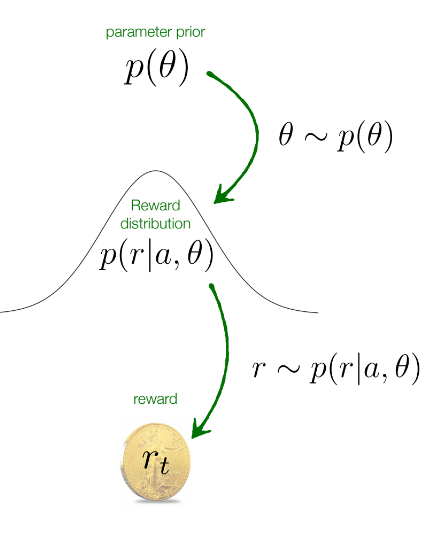
\includegraphics[scale=0.4]{images/bayesian_stochastic_bandits.png}
    \caption{Bayesian Stochastic Bandits}
    \label{fig:bayesian_bandits}
\end{figure}


\subsection{Thompson Sampling}

Thomson Sampling requires assuming a Bayesian Stochastic Bandit. In other words, it assumes that the reward is generated from a distribution which is parameterized by $\theta$. Since $\theta$ isn't directly observable and hence unknown, it maintains a running estimate of $\theta$, denoted by $\hat{\theta}$, by observing the rewards. To select the arm to pull, we select the arm with the highest expected reward. Mathematically:

$$a = \arg \max_k \mathbb{E}_{p(r|a_k, \hat{\theta}_k)}\left[r|a_k, \hat{\theta}_k\right]$$

In case the actual $\theta^*$ was known, we could simply replace $\hat{\theta}$ with $\theta^*$ in the above equation.

\subsubsection{Estimating $\theta$}

To estimate the true parameter $\theta$, we would use a history of actions taken and reward received to condition the parameter. The argument is very similar to a maximum likelihood (MLE) argument, or strictly maximum-a-posteriori (MAP) in our case. We wish to obtain an estimate $\hat{\theta}$ that maximizes the likelihood of observing the history of actions and rewards. Mathematically,

$$p(\theta | h^{(t)}) = p(\theta | a^{(1)}, r^{(1)}, \dots, a^{(t)}, r^{(t)})$$
$$\hat{\theta} = \arg \max_{\theta} p(\theta|h^{(t)})$$

where $h^{(t)} =\{a^{(1)}, r^{(1)}, \dots, a^{(t)}, r^{(t)}\}$ is the history of actions and rewards.

Now that we know how we are going to get the estimate for $\theta$. Lets see how we can compute the estimate $\hat{\theta}$.

Using Bayes rule:
$$p(\theta | a^{(1)}, r^{(1)}, \dots, a^{(t)}, r^{(t)}) = \frac{p(r^{(1)}, \dots, r^{(t)} | \theta, a^{(1)}, \dots, a^{(t)})p(\theta | a^{(1)}, \dots, a^{(t)})}{p(r^{(1)}, \dots, r^{(t)} | a^{(1)}, \dots, a^{(t)})}$$

\normalfont
\begin{figure}[t]
    \centering
    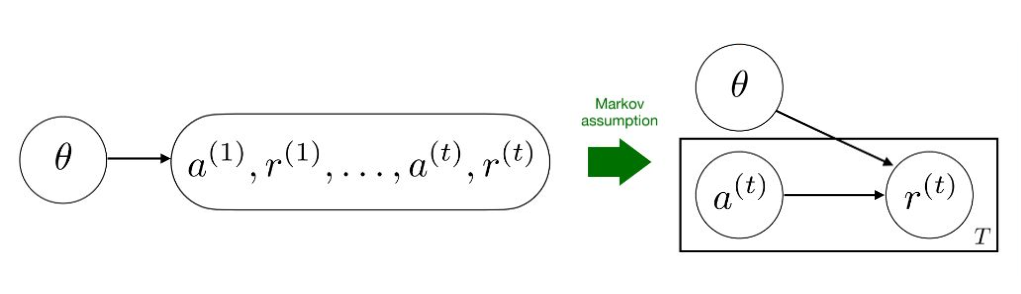
\includegraphics[scale=0.6]{images/markov.pdf}
    \caption{$r^{(t)}$ is dependent on $a^{(t)}$ and $\theta$, while $a^{(t)}$ and $\theta$ are independent}
    \label{fig:plate}
\end{figure}

Now in a bandit setting, the next state is independent of the actions taken by a learner. In other words, $\theta$ is independent of all $a^{(t)}$'s.

$$p(\theta | a^{(1)}, r^{(1)}, \dots, a^{(t)}, r^{(t)}) = \frac{p(r^{(1)}, \dots, r^{(t)} | \theta, a^{(1)}, \dots, a^{(t)})p(\theta)}{p(r^{(1)}, \dots, r^{(t)} | a^{(1)}, \dots, a^{(t)})}$$

Assuming that the reward $r^{(t)}$ is conditionally independent of other rewards given the action and the parameter $\theta$, ie. rewards are i.i.d. We have,

$$p(\theta | a^{(1)}, r^{(1)}, \dots, a^{(t)}, r^{(t)}) = \frac{\prod_t  p(r^{(t)} | \theta, a^{(1)}, \dots, a^{(t)})p(\theta)}{\prod_t p(r^{(t)} | a^{(1)}, \dots, a^{(t)})}$$ 

Now, using Markov assumption $p(r^{(t)} | \theta, a^{(1)}, \dots, a^{(t)} = p(r^{(t)} | \theta, a^{(t)})$:
$$p(\theta | a^{(1)}, r^{(1)}, \dots, a^{(t)}, r^{(t)}) = \frac{\prod_t  p(r^{(t)} | \theta, a^{(t)}p(\theta)}{\prod_t p(r^{(t)} | a^{(t)})}$$ 

Thus the posterior distribution simplifies to:
$$p(\theta | h^{(t)}) \propto \prod_t  p(r^{(t)} | \theta, a^{(t)}p(\theta)$$ 

which can be written in an incremental fashion:
$$p(\theta | h^{(t)}) \propto p(r^{(t)} | \theta, a^{(t)}p(\theta|h^{(t-1)})$$

Now that we have an incremental update to the posterior $p(\theta|h^{(t)}$, we use this to obtain our estimate $\hat{\theta}_k$ for the $k^{th}$ arm as:

$$\hat{\theta}_k = \arg \max_{\theta_k} p(\theta_k | h_k^{(t)})$$
$$\hat{\theta}_k = \arg \max_{\theta_k} \underbrace{p(r^{(t)} | a_k^{(t)}, \theta_k)}_{\text{likelihood}}\underbrace{p(\theta_k|h_k^{t-1})}_{\text{prior}}$$

In the above equation, we can replace $r^{(t)}$ with $r^{(t)}_k$ which would mean the same thing. Here, it's implicit that the reward $r^{(t)}$ is obtained after picking arm $k$.

We can greatly simplify the complex posterior updates by assuming certain distributions for prior and likelihood, which is covered in the next section.

\subsubsection{Conjugate Priors}
\begin{figure}[H]
    \centering
    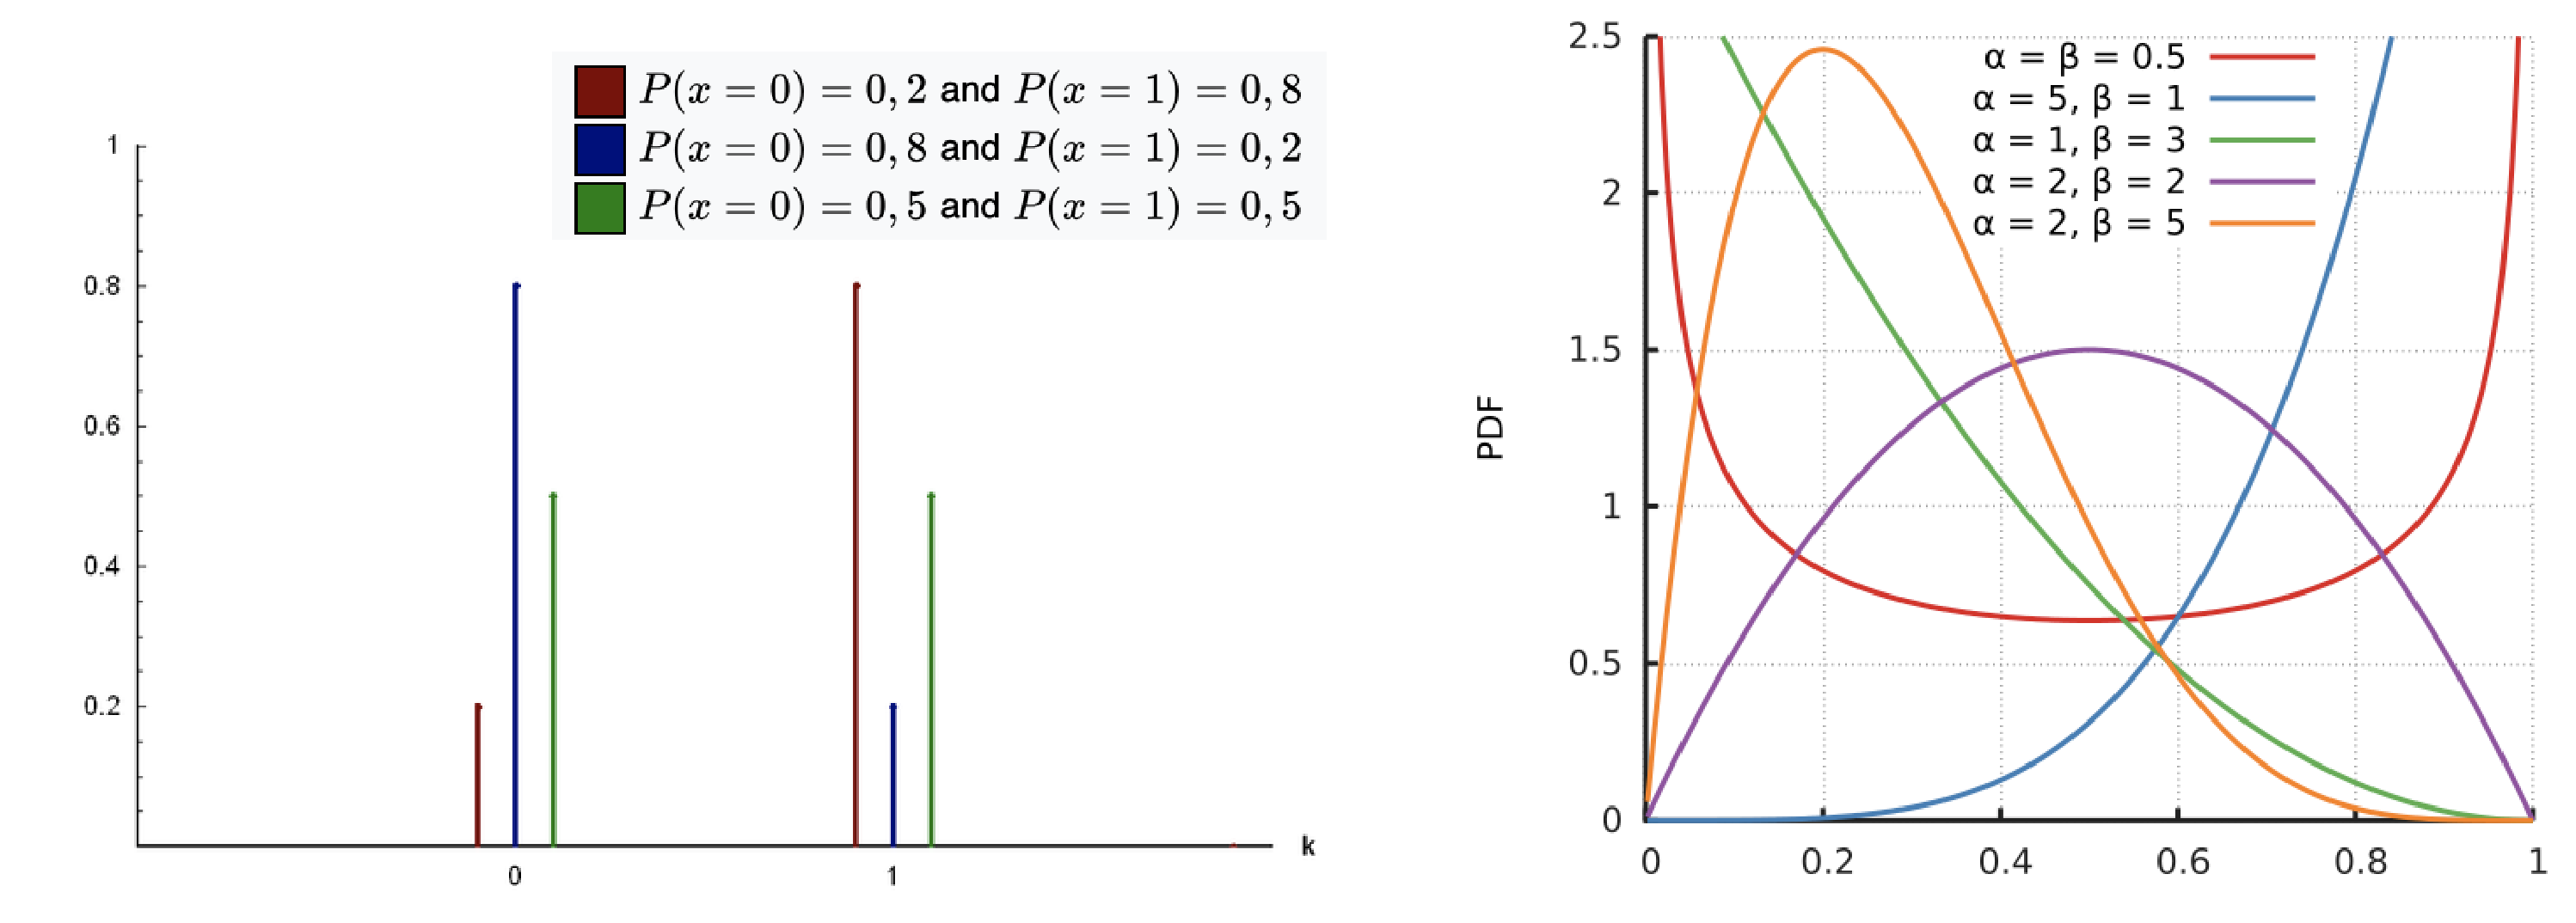
\includegraphics[width=\textwidth]{images/beta-bernoulli.png}
    \caption{Conjugate Priors. Beta distribution (right) is a conjugate prior of the Bernoulli
    distribution (left).}
    \label{fig:my_label}
\end{figure}
Consider the general posterior estimation scenario:
\[
\underbrace{p(\theta \mid x)}_{\text{posterior}} \propto \underbrace{p(x \mid \theta)}_{\text{likelihood}} \underbrace{p(\theta)}_{\text{prior}}
\]
When the posterior and the prior have the same type of distribution, they are called
\textit{conjugate distributions}. In this case, the prior is called a \textit{conjugate prior}.
For example, the Beta distribution is the conjugate prior of the Bernoulli distribution:
\begin{align*}
p(r \mid \theta) &= \theta^r (1-\theta)^{1-r} \tag{Bernoulli Distribution}\\
p(\theta) &= \frac{\Gamma(\alpha + \beta)}{\Gamma(\alpha) \Gamma(\beta)} \theta^{\alpha - 1} (1 - \theta)^{\beta - 1} \tag{Beta Distribution}
\end{align*}
where $\Gamma(n) = (n-1)!$ is the Gamma function. We can easily show that posterior is Beta
distribution if the \textit{likelihood} is a Bernoulli distribution and \textit{prior} is
a Beta distribution.
\begin{align*}
    p(\theta \mid r) &\propto p(r \mid \theta) p(\theta)\\
    &\propto \theta^r(1-\theta)^{1-r} \theta^{\alpha - 1} (1-\theta)^{\beta - 1}\\
    &\propto \theta^{(r + \alpha - 1)}(1-\theta)^{(1-r+\beta) - 1} \\
    &\propto \theta^{(\alpha' - 1)}(1-\theta)^{\beta' - 1}
\end{align*}
We observe that the posterior can be calculated efficiently via additive updates:
\begin{align*}
    \beta' &= \beta + 1 - r\\
    \alpha' &= \alpha + r.
\end{align*}

Thus, we can use the conjugate distributions to design an efficient strategy to update the
\textit{maximum-a-posteriori} estimate for $\theta$. We now study the generic algorithm for
Thompson Sampling followed by a specific example that uses Beta conjugate prior for Bernoulli
likelihood.

\subsubsection{Thompson Sampling Algorithm: Generic and Bern-Beta}
The generic algorithm for Thompson Sampling \cite{thompson1933likelihood} is shown in
Alg. \ref{algo:thompson_sampling_generic}.
\begin{algorithm}
\caption{Thompson Sampling (Incremental)}
\label{algo:thompson_sampling_generic}
\begin{algorithmic}[1]
\FOR{$t=1 \rightarrow T$}
\STATE $\theta_k \sim p(\theta_k \mid h_k)$ \hfill $\triangleright$ sample from posterior
\STATE $a_{\hat{k}}^{(t)} = \arg \max_k \mathbb{E}_{p(r \mid a_k, \theta_k)} [r \mid a_k, \theta_k]$ \hfill $\triangleright$ predict
\STATE Receive($r^{(t)}$) \hfill $\triangleright$ get sampled reward
\STATE $p(\theta_{\hat{k}} \mid h_{\hat{k}}) \propto p(r^{(t)} \mid a_{\hat{k}}^{(t)}, \theta_{\hat{k}} p(\theta_{\hat{k}} \mid h_{\hat{k}}))$ \hfill $\triangleright$ update posterior
\ENDFOR
\end{algorithmic}
\end{algorithm}

Let us understand this generic algorithm with the Bernoulli-Beta case. The algorithm proceeds
as shown in Alg. \ref{algo:bern_beta_thompson}.
\begin{algorithm}
\caption{Bern-Beta Thompson Sampling}
\label{algo:bern_beta_thompson}
\begin{algorithmic}[1]
\FOR{$t=1 \rightarrow T$}
\STATE $\theta_k \sim p(\theta_k; \alpha_k, \beta_k)$ \hfill $\triangleright$ sample from posterior
\STATE $a_{\hat{k}}^{(t)} = \arg \max_k \mathbb{E}_{p(r \mid a_k, \theta_k)} [r \mid a_k, \theta_k]$ \hfill $\triangleright$ predict
\STATE Receive($r^{(t)}$) \hfill $\triangleright$ get sampled reward
\STATE  $\alpha_{\hat{k}} = \alpha_{\hat{k}} + r^{(t)}$\hfill $\triangleright$ update posterior
\STATE  $\beta_{\hat{k}} = \beta_{\hat{k}} + 1 - r^{(t)}$\hfill $\triangleright$ update posterior
\ENDFOR
\end{algorithmic}
\end{algorithm}

For each time step $t$, first a parameter estimate $\theta_k$ is sampled from the posterior
$p(\theta_k; \alpha_k, \beta_k)$ for all arms $k = \{ 1, \ldots, K \}$. Then, the action
$a_{\hat{k}}^{(t)}$ is picked that maximized the expected reward over the arms. After pulling
the arm we get some reward at this time step, $r^{(t)}$. Using this reward, the posterior
is updated by changing $\alpha_{\hat{k}}$ and $\beta_{\hat{k}}$ for the arm that was pulled.
The process repeats for all the time steps.

\subsubsection{Empirical Performance Comparison with UCB}
\begin{figure}[t]
    \centering
    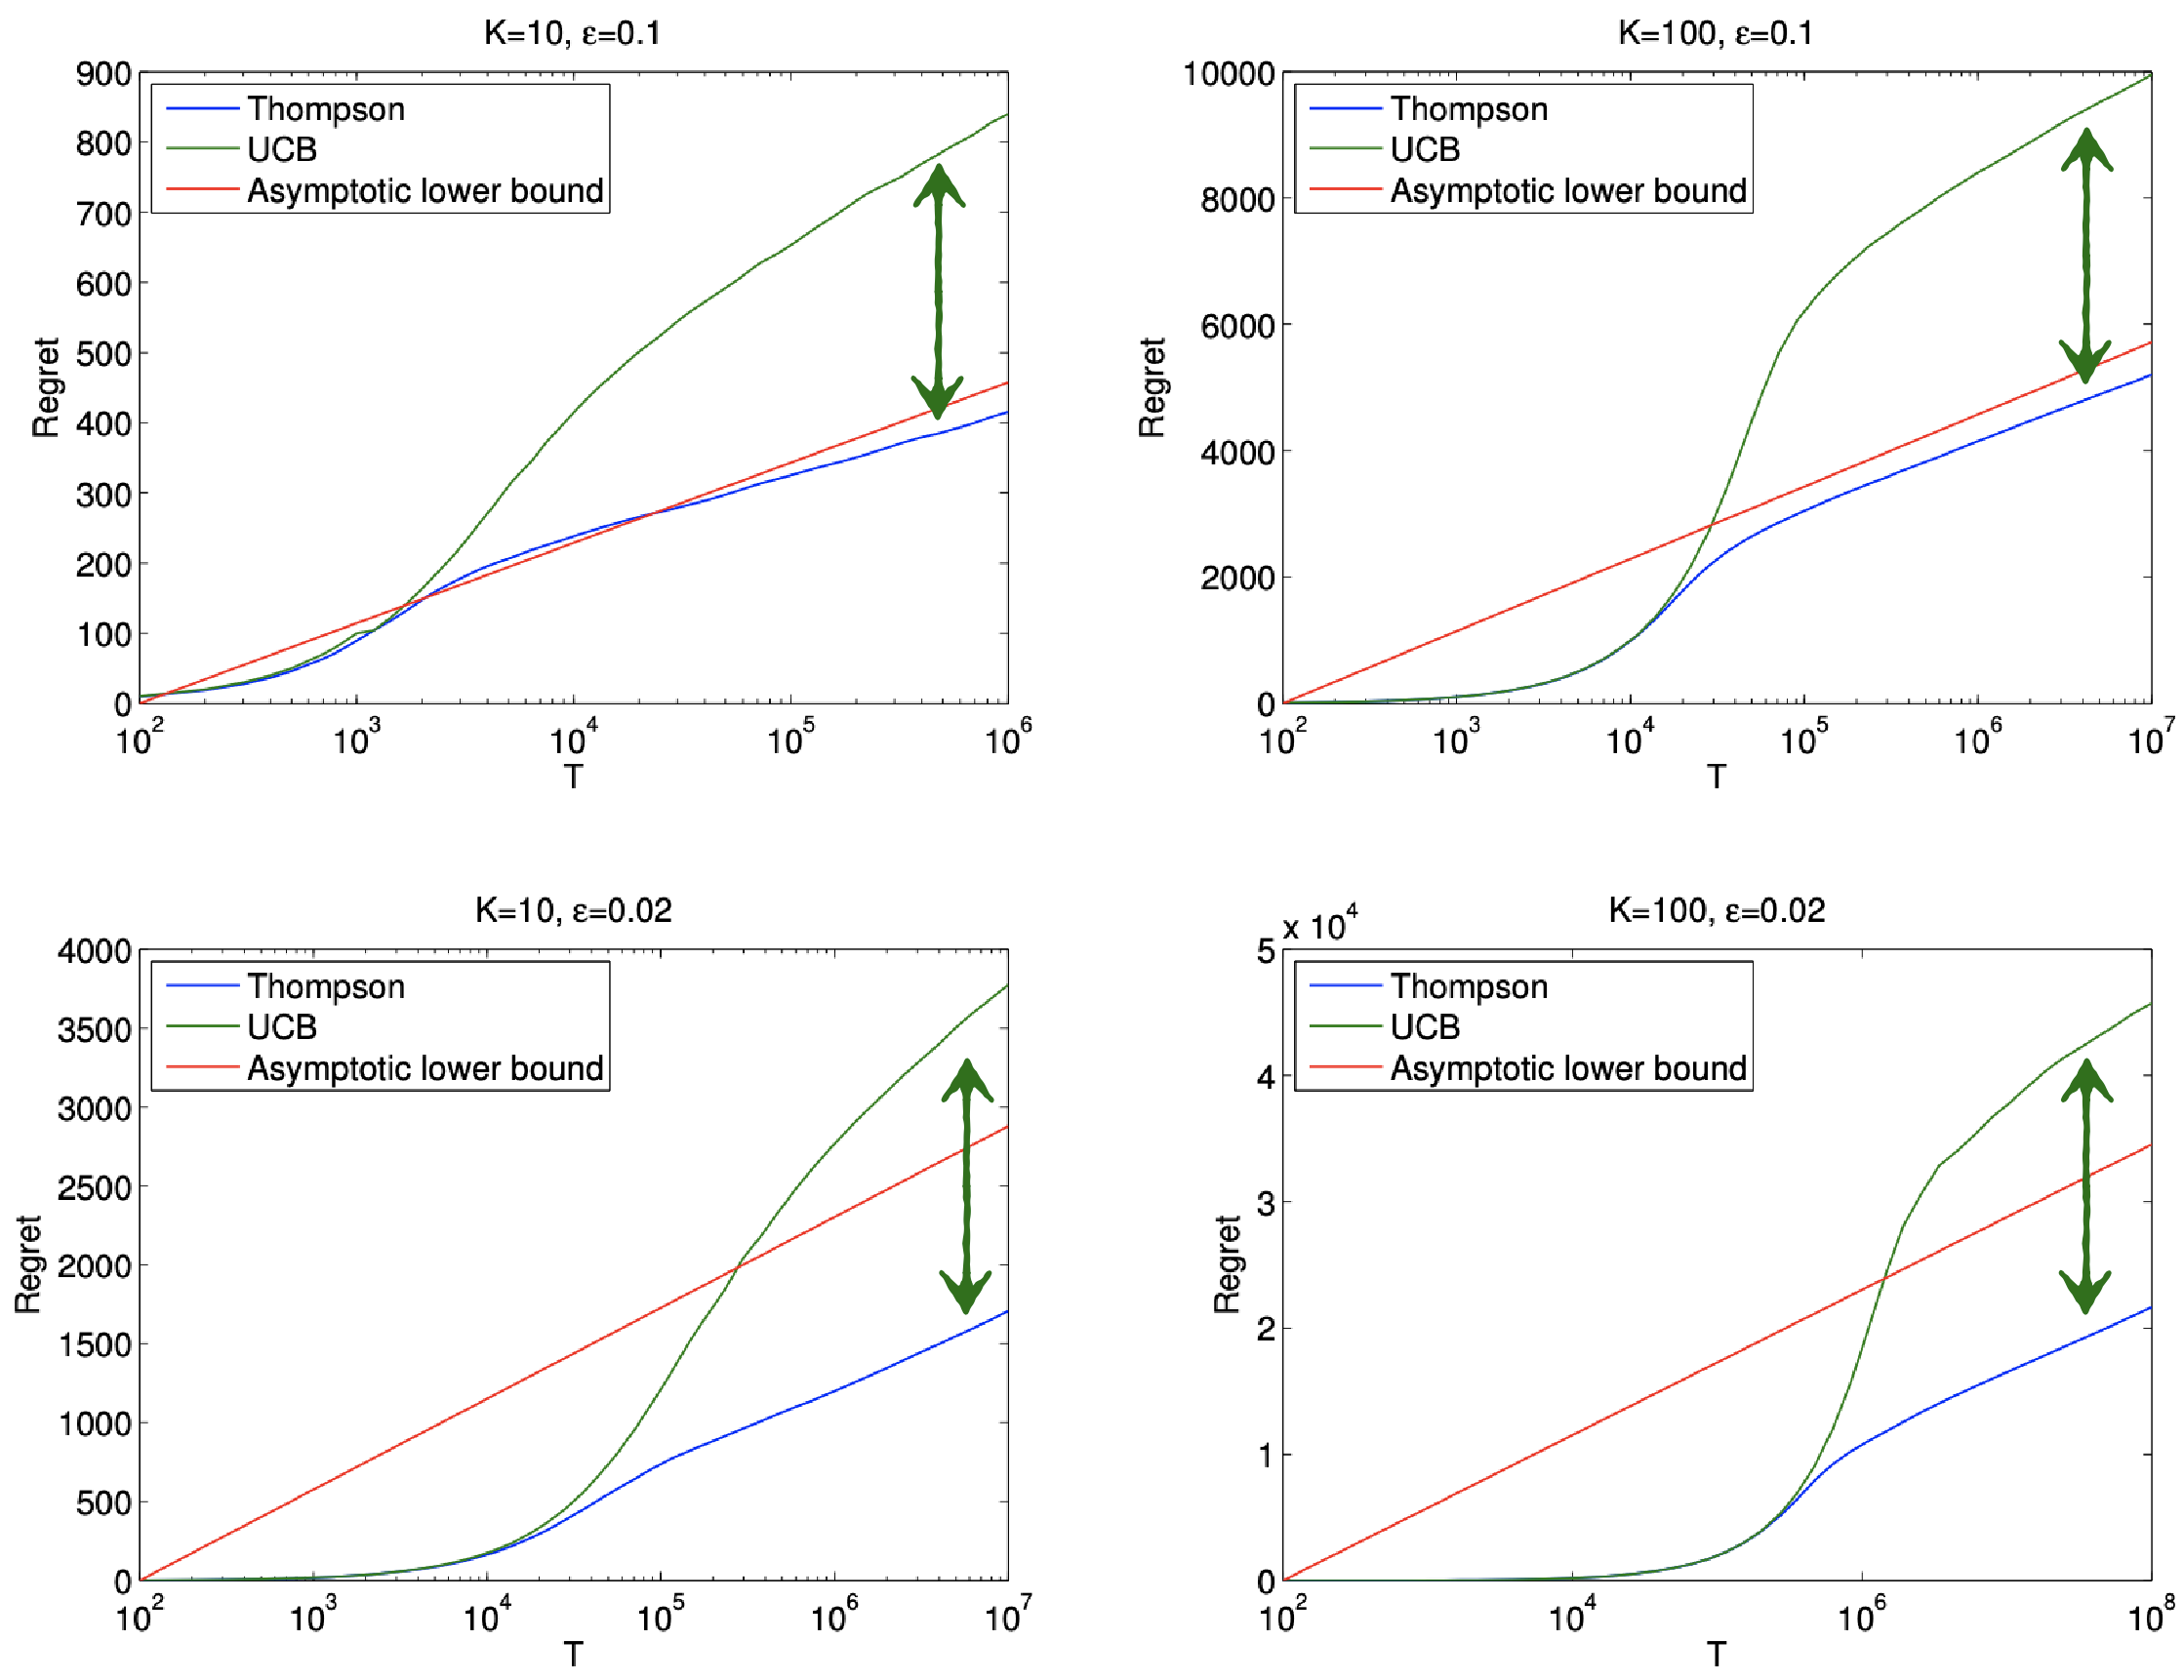
\includegraphics[width=\textwidth]{images/beta-bernoulli-empirical.png}
    \caption{Empirical performance comparison between Thompson Sampling and the UCB algorithms \cite{chapelle2011empirical}.}
    \label{fig:empirical_perf}
\end{figure}

Empirically, \cite{chapelle2011empirical} provides an empirical performance comparison of
the Thompson Sampling algorithm with respect to the UCB algorithm
(Fig. \ref{fig:empirical_perf}). It is observed that Thompson sampling has a lower regret than UCB, especially when the timesteps is large. This effect is true for different values of the number of arms $K$, and the $\epsilon$.

Interestingly, it performs better than the asymptotic lower bound:

$$\mathcal{R}(T) \ge \log(T)\left[\sum_{i=1}^K \frac{p^* - p_i}{D(p_i || p^*)} + O(1)\right]$$
Theoretically, the regret for Thompson Sampling is known to be $\mathcal{R}(T) = \mathcal{O}(\sqrt{KT \log T})$.

where $p^* = \max p_i$ and $D(p_i || p^*)$ is the KL-divergence between $p_i$ and $p^*$.

% Bandits is exhaustive but Contextual is not why?

%\section*{References}
%Include your references here. Please cite any resources you found useful.	
%Populate the refs.bib file or list your references manually. Be consistent in formatting!
{
\bibliography{refs}
\bibliographystyle{abbrv}
}

%\section{Appendix}
%This section provides any relevant background material that was not covered in the lectures, but was found to be useful for understanding the material. 
%For example, derivations, theory underlying techniques employed, etc. 

%Additionally, this section can summarizes applications or extensions of these techniques found in the literature. 

\end{document} % Done!


